% Generated by analysis/plot_results.py; edit that file to regenerate.
\centering

\includegraphics[width=1.0000\linewidth]{figures/data_app_necessity_legend.pdf}
\par\vspace{1pt}
\begin{subfigure}[t]{0.3260\linewidth}
\centering
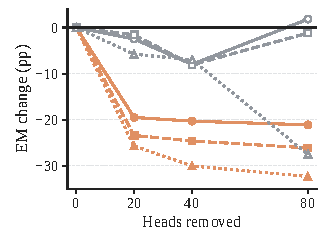
\includegraphics[width=\linewidth]{figures/data_app_necessity_a.pdf}
\caption{Composed}
\label{fig:data-app-necessity-a}
\end{subfigure}%
\hfill%
\begin{subfigure}[t]{0.3260\linewidth}
\centering
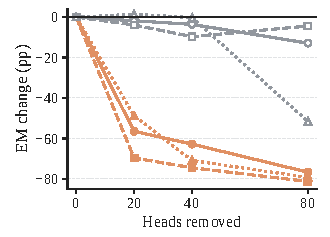
\includegraphics[width=\linewidth]{figures/data_app_necessity_b.pdf}
\caption{First hop}
\label{fig:data-app-necessity-b}
\end{subfigure}%
\hfill%
\begin{subfigure}[t]{0.3260\linewidth}
\centering
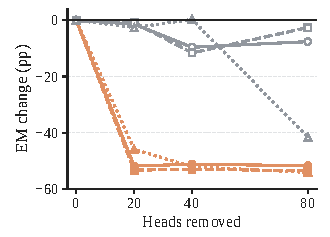
\includegraphics[width=\linewidth]{figures/data_app_necessity_c.pdf}
\caption{Second hop}
\label{fig:data-app-necessity-c}
\end{subfigure}%
\par
